\documentclass{article}
\usepackage{iclr2027_conference,times}

\usepackage{amsmath,amssymb,amsthm}
\usepackage{booktabs}
\usepackage{graphicx}
\usepackage{microtype}
\usepackage{xcolor}
\usepackage{url}
\usepackage{algorithm}
\usepackage{algorithmic}
\usepackage{flafter}
\usepackage{placeins}
\usepackage[hidelinks]{hyperref}

\graphicspath{{figures/}}

\newcommand{\E}{\mathbb{E}}
\newcommand{\R}{\mathbb{R}}
\newcommand{\M}{\mathcal{M}}
\newcommand{\dproxy}{\Delta_V}
\newcommand{\dtrue}{\Delta_*}
\newcommand{\pii}{\pi}
\newcommand{\pip}{\pi'}
\newtheorem{proposition}{Proposition}
% Generated by scripts/build_paper_snippets.py; do not edit by hand.
\newcommand{\OperatorShiftSeeds}{30}
\newcommand{\OperatorShiftRows}{36000}
\newcommand{\OperatorShiftEffect}{0.2627}
\newcommand{\OperatorShiftEffectCI}{[0.1684,\,0.3763]}
\newcommand{\ClosedLoopSeeds}{30}
\newcommand{\ClosedLoopRounds}{40}
\newcommand{\ClosedLoopProxyCISR}{0.0253}
\newcommand{\ClosedLoopPivotCISR}{0.0981}
\newcommand{\ClosedLoopPerformativeProxyCISR}{4.2631}
\newcommand{\ClosedLoopPerformativePivotCISR}{1.2136}
\newcommand{\ClosedLoopEffect}{1.4883}
\newcommand{\ClosedLoopEffectCI}{[1.0618,\,1.9105]}
\newcommand{\OODSeeds}{30}
\newcommand{\OODRows}{36000}
\newcommand{\OODGain}{-0.2590}
\newcommand{\OODGainCI}{[-0.3588,\,-0.1707]}
\newcommand{\EfficiencySeeds}{30}
\newcommand{\EfficiencyPairedN}{180}
\newcommand{\EfficiencyEffect}{0.000668}
\newcommand{\EfficiencyEffectCI}{[0.000011,\,0.0013]}
\newcommand{\StrategicSeeds}{30}
\newcommand{\StrategicClusters}{30}
\newcommand{\StrategicAdaptiveFamilies}{3}
\newcommand{\StrategicFamilySeedTraces}{90}
\newcommand{\StrategicEffect}{-0.0240}
\newcommand{\StrategicEffectCI}{[-0.0249,\,-0.0231]}
\newcommand{\StrategicReversalRate}{0.9495}
\newcommand{\StrategicSIRR}{0.9495}
% Strategic effect: mean of three adaptive family values within each matched seed; interval bootstraps matched seeds.
% Strategic reversal rate: unweighted mean of the three family-level SIRRs.
% The external finance audit is observational and has no causal reversal estimate.
\newcommand{\StrategicAllFamilySeedTraces}{150}

% Generated by scripts/build_revision_evidence.py; do not edit.
\newcommand{\RevisionLeducHtwo}{0.036}
\newcommand{\RevisionLeducHtwoCI}{[0.014, 0.064]}
\newcommand{\RevisionLeducHthree}{0.036}
\newcommand{\RevisionLeducPivotISR}{0.009}
\newcommand{\RevisionLeducUniformISR}{0.046}
\newcommand{\RevisionLeducAllHFISR}{0.009}
\newcommand{\RevisionLeducNoHFISR}{0.094}
\newcommand{\RevisionLeducCostShare}{0.22}
\newcommand{\RevisionVFourHtwo}{0.906}
\newcommand{\RevisionVFourHtwoCI}{[-0.784, 3.401]}
\newcommand{\RevisionVFourHthree}{1.481}
\newcommand{\RevisionVFourHthreeCI}{[-0.393, 4.096]}
\newcommand{\RevisionVFourOneQuery}{3.423}
\newcommand{\RevisionVFourOneQueryCI}{[0.390, 6.944]}
\newcommand{\RevisionVFourShort}{-0.575}
\newcommand{\RevisionVFourShortCI}{[-1.042, -0.180]}
\newcommand{\RevisionVFourPivotISR}{0.836}
\newcommand{\RevisionVFourUniformISR}{1.742}
\newcommand{\RevisionVFourAllHFISR}{0.750}
\newcommand{\RevisionVFourNoHFISR}{10.339}
\newcommand{\RevisionVFourCostShare}{0.29}
\newcommand{\RevisionKuhnHtwo}{0.002}
\newcommand{\RevisionKuhnHtwoCI}{[0.000, 0.006]}
\newcommand{\RevisionKuhnPivotISR}{0.056}
\newcommand{\RevisionKuhnUniformISR}{0.058}
\newcommand{\RevisionLeducResponseGap}{1.704}
\newcommand{\RevisionLeducResponseGapCI}{[1.315, 2.127]}
\newcommand{\RevisionLeducNormalizedResponseGap}{0.57}
\newcommand{\RevisionLeducNormalizedResponseGapCI}{[0.45, 0.70]}
\newcommand{\RevisionLeducIDE}{1.016}
\newcommand{\RevisionLeducIRR}{0.500}
\newcommand{\RevisionLeducISC}{0.556}
\newcommand{\RevisionKuhnResponseGap}{0.080}
\newcommand{\RevisionKuhnResponseGapCI}{[0.056, 0.106]}
\newcommand{\RevisionKuhnNormalizedResponseGap}{0.50}
\newcommand{\RevisionKuhnNormalizedResponseGapCI}{[0.38, 0.62]}
\newcommand{\RevisionKuhnIDE}{0.219}
\newcommand{\RevisionKuhnIRR}{0.471}
\newcommand{\RevisionKuhnISC}{0.581}
\newcommand{\RevisionVFourResponseGap}{50.881}
\newcommand{\RevisionVFourResponseGapCI}{[40.495, 62.823]}
\newcommand{\RevisionVFourNormalizedResponseGap}{0.13}
\newcommand{\RevisionVFourNormalizedResponseGapCI}{[0.10, 0.17]}
\newcommand{\RevisionVFourIDE}{6.840}
\newcommand{\RevisionVFourIRR}{0.550}
\newcommand{\RevisionVFourISC}{0.383}
\newcommand{\RevisionHomogeneousGap}{98.3}
\newcommand{\RevisionHomogeneousGapCI}{[77.2, 123.4]}
\newcommand{\RevisionHomogeneousEffect}{-1.600}
\newcommand{\RevisionHomogeneousEffectCI}{[-5.235, 1.946]}
\newcommand{\RevisionMPEPushResponse}{0.005}
\newcommand{\RevisionMPEPushResponseCI}{[-0.004, 0.015]}
\newcommand{\RevisionMPEAdversaryResponse}{-0.039}
\newcommand{\RevisionMPEAdversaryResponseCI}{[-0.093, 0.015]}
\newcommand{\RevisionDecisionRoots}{90}
\newcommand{\RevisionDecisionFlips}{51}
\newcommand{\RevisionDecisionStable}{39}
\newcommand{\RevisionFlippedNormalizedGain}{0.075}
\newcommand{\RevisionFlippedNormalizedGainCI}{[0.004, 0.157]}
\newcommand{\RevisionStableNormalizedGain}{0.140}
\newcommand{\RevisionStableNormalizedGainCI}{[0.049, 0.250]}
\newcommand{\RevisionCriticalQueryRate}{0.97}
\newcommand{\RevisionCriticalQueryRateCI}{[0.92, 1.00]}
\newcommand{\RevisionCriticalQueryHitGain}{0.113}
\newcommand{\RevisionCriticalQueryHitGainCI}{[0.055, 0.180]}
\newcommand{\RevisionCriticalQueryMissGain}{-0.195}
\newcommand{\RevisionCriticalQueryMissGainCI}{[-0.584, 0.000]}
\newcommand{\RevisionCriticalNoiseMargin}{13.99}
\newcommand{\RevisionCriticalNoiseMarginCI}{[7.97, 22.90]}
\newcommand{\RevisionPostQuerySeparation}{0.06}
\newcommand{\RevisionPostQuerySeparationCI}{[0.05, 0.08]}
\newcommand{\RevisionLeducFlips}{18}
\newcommand{\RevisionKuhnFlips}{14}
\newcommand{\RevisionMeltingFlips}{19}
\newcommand{\RevisionLeducCriticalQueryRate}{1.00}
\newcommand{\RevisionKuhnCriticalQueryRate}{1.00}
\newcommand{\RevisionMeltingCriticalQueryRate}{0.90}

% Generated from hash-checked paired seed evidence.
\newcommand{\HighwayCalibrationSeeds}{20}
\newcommand{\HighwaySeeds}{60}
\newcommand{\HighwayCandidateCount}{5}
\newcommand{\HighwayQueryRows}{1560}
\newcommand{\HighwayTruthRows}{3000}
\newcommand{\HighwayBudgetOneContrast}{$-0.0226$}
\newcommand{\HighwayBudgetOneCI}{$[-0.0439,-0.0008]$}
\newcommand{\HighwayBudgetTwoContrast}{$0.0049$}
\newcommand{\HighwayBudgetTwoCI}{$[-0.0088,0.0199]$}
\newcommand{\HighwayBudgetFourContrast}{$0.0115$}
\newcommand{\HighwayBudgetFourCI}{$[0.0008,0.0237]$}
\newcommand{\HighwayReplicationCalibrationSeeds}{20}
\newcommand{\HighwayReplicationSeeds}{60}
\newcommand{\HighwayReplicationCandidateCount}{5}
\newcommand{\HighwayReplicationQueryRows}{1380}
\newcommand{\HighwayReplicationTruthRows}{2100}
\newcommand{\HighwayReplicationBudgetTwoContrast}{$-0.0006$}
\newcommand{\HighwayReplicationBudgetTwoCI}{$[-0.0143,0.0145]$}
\newcommand{\HighwayReplicationBudgetFourContrast}{$0.0034$}
\newcommand{\HighwayReplicationBudgetFourCI}{$[-0.0007,0.0099]$}
\newcommand{\HighwayRedesignCalibrationSeeds}{40}
\newcommand{\HighwayRedesignSeeds}{120}
\newcommand{\HighwayRedesignCandidateCount}{8}
\newcommand{\HighwayRedesignQueryRows}{720}
\newcommand{\HighwayRedesignTruthRows}{1080}
\newcommand{\HighwayRedesignBudgetTwoContrast}{$0.0456$}
\newcommand{\HighwayRedesignBudgetTwoCI}{$[0.0343,0.0587]$}
\newcommand{\HighwayRedesignBudgetFourContrast}{$0.0380$}
\newcommand{\HighwayRedesignBudgetFourCI}{$[0.0300,0.0474]$}


\title{When Better Gets Worse:\\
Improvement Fidelity for Self-Improving Agents in\\
Adaptive Worlds}
\author{}
\date{}

\begin{document}
\maketitle

\begin{abstract}
We study a replacement transition in which an improvement operator proposes
policy candidates, a proxy verifier scores them, and deployment changes the
world in which they are evaluated. An update that looks better to the verifier
can therefore become worse after deployment even when the verifier ranks
policies well overall.
We formalize this gap as \emph{Improvement Fidelity}, our core evaluation
target: whether proxy improvements preserve the sign and ordering of deployment
improvements over the updates an improvement process proposes. We show that
global policy accuracy need not guarantee update fidelity: operator shift and
deployment response can create update-level errors, while candidate margins
determine whether those errors change the replacement decision. PIVOT is the
paired validation framework; \textbf{PIVOT-KG} is a concrete application of
the established one-step correlated-Gaussian knowledge gradient that allocates
scarce high-fidelity evaluation according to expected reduction in selection
regret per unit cost. Across 90 held-out roots in Leduc, Kuhn, and Melting Pot,
proxy and deployment optimal sets are disjoint in 51 cases. In an
eight-candidate HighwayEnv saved-truth replay, PIVOT-KG reduces mean
improvement-selection regret from 0.0435 under exact Uniform validation
to 0.0055 at the primary budget. Together, these results show why
operator-proposed replacements should be evaluated in the worlds they induce,
while testing an allocation rule for cases in which scarce deployment evidence
can affect the replacement decision.\footnote{Our code is available at \urlstyle{same}\url{https://anonymous.4open.science/r/pivot-anonymous-review-2E67/}.}
\end{abstract}


\section{Introduction}

An improvement operator can repeatedly propose candidate policies, score them
with a verifier, and deploy a replacement. Yet an update that looks better to the
verifier can become worse after deployment when the deployed policy changes the
world in which it is evaluated. A lane change alters nearby trajectories, and
an action in a multi-agent game changes how other agents respond. A verifier
can therefore be accurate over policies in aggregate and still choose the wrong
local replacement. Figure~\ref{fig:reversal} illustrates this failure mode.

\begin{figure}[t]
  \centering
  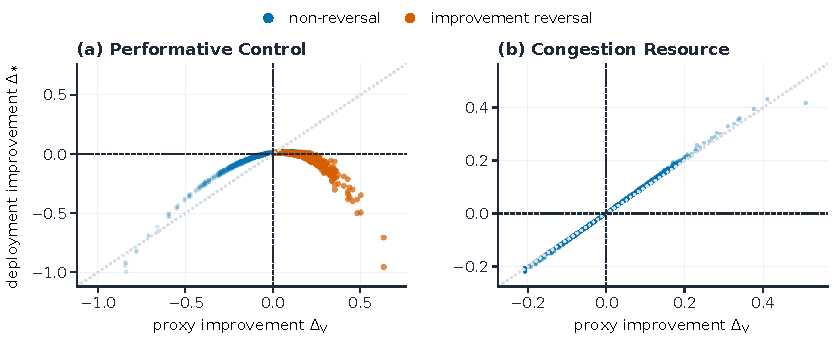
\includegraphics[width=\linewidth]{fig1_improvement_reversal.pdf}
  \caption{Proxy improvements can reverse after deployment. Each point is a
  proposed update; lower-right points are proxy-positive but
  deployment-negative.}
  \label{fig:reversal}
\end{figure}

We call this transition-level requirement \emph{Improvement Fidelity}: whether
an improvement under the verifier remains an improvement after deployment in
the world induced by the update. Because deployment evaluation is often too
costly for every candidate, we instantiate PIVOT (Paired Interventional
Validation of Optimization Transitions) with \textbf{PIVOT-KG}, a standard
correlated-Gaussian knowledge-gradient validator that directs a limited
high-fidelity (HF) budget to uncertainty that can change the replacement
decision.

Prior work separately studies deployment-induced response, policy-level
evaluation or safe improvement, and verifier reliability. We instead study an
operator-relative criterion for whether a proposed replacement remains an
improvement in the world it induces, together with a decision-aware rule for
allocating scarce deployment evidence for that decision.
Our analysis treats decision preservation under differential error as a
margin-dependent property of each replacement operation proposed by the
improvement operator.

PIVOT is the paired validation framework for this replacement problem, whereas
PIVOT-KG is one concrete instantiation using the established one-step
correlated-Gaussian knowledge-gradient rule. We therefore claim neither a new
KG acquisition theorem nor a general policy-improvement algorithm: the
algorithmic question is when decision-aware HF allocation adds value for the
operator's proposed transition.

\FloatBarrier

Our contributions are:

\noindent\textbf{1. Improvement Fidelity.}
We formulate operator-proposed replacement as an operator-relative,
transition-level
evaluation problem and introduce Improvement Fidelity, showing why strong global
policy evaluation need not imply reliable evaluation of the updates an agent
actually proposes.

\smallskip
\noindent\textbf{2. PIVOT validation framework and standard-KG instantiation.}
PIVOT defines paired, operator-relative validation; PIVOT-KG applies an
established correlated-Gaussian KG rule to allocate limited HF evidence by its
expected reduction in update-selection regret rather than global prediction
error.

\smallskip
\noindent\textbf{3. Evidence across response worlds.}
Across controlled response worlds, multi-agent environments, and reactive
driving simulations, we test the failure mechanisms predicted by the
theory and identify when targeted HF validation reduces selection regret.

\smallskip

Together, these contributions shift the evaluation of proposed replacement from
whether policies are evaluated accurately in a proxy world to whether proposed
improvements remain improvements after deployment, while providing a principled
basis for allocating deployment evidence when it can affect the replacement decision.

\section{Related Work}

\paragraph{Performative and strategic response.}
Performative prediction and reinforcement learning study settings in which
deployment changes the data distribution, dynamics, rewards, or behavior of
other agents
~\citep{perdomo2020performative,mandal2023performative,rank2024performative,
mandal2025linear,gois2025performative,multiagentperformative2022}.
These works study how deployment-induced response affects learning, stability,
and optimality. We instead ask a local evaluation question: whether a
particular proposed replacement remains an improvement under the response
world it induces.

\paragraph{Policy evaluation and safe improvement.}
Off-policy evaluation and safe policy improvement estimate or certify the
performance of a candidate relative to a baseline
~\citep{jiang2016doubly,thomas2015hcpi,laroche2019spibb}, while
work on learned simulators studies policy evaluation, policy-value gaps,
or ranking preservation~\citep{worldgym2025,policyaware2026}.
Our focus is the proposed transition itself: a proxy can preserve policy-level
accuracy or rankings yet still induce the wrong local replacement decision
once deployment changes the evaluation world.

\paragraph{Self-improvement and verification.}
Recent work has made iterative policy or agent improvement operational
~\citep{evopolicygym2026,dgm2025} and has documented regressions or failures of
verification during self-improvement
~\citep{wu2024progress,selfauthored2026}. Related work on reward
overoptimization shows that optimizing an imperfect proxy can itself degrade
true performance~\citep{gao2023reward,laidlaw2025correlated}.
Our failure mode is complementary: the verifier need not be self-authored,
changing, or directly exploited. Even a fixed external verifier can select the
wrong update when deployment changes the world in which that update is
evaluated.

\paragraph{Adaptive selection and paired evaluation.}
Knowledge-gradient, ranking-and-selection, and best-arm methods allocate costly
observations to decision-relevant alternatives under limited budgets
~\citep{chick2001crn,frazier2009kg,kalyanakrishnan2012pac,xie2016pairwise,konyushova2021active}.
PIVOT-KG instantiates established KG for operator-relative replacement
validation; unlike Active Offline Policy Selection, it targets candidate-dependent
deployment worlds and proxy-to-deployment replacement regret, while
introducing no new KG acquisition rule.

\paragraph{Scope relative to adjacent fields.}
These literatures motivate our setting but target different objects. Game
theory studies strategic interaction and equilibrium concepts, while
performative prediction studies distributional response and often fixed-point
or learning behavior. PIVOT asks the narrower deployment decision question:
given one operator-proposed replacement, does it remain worth deploying in the
world induced by that replacement? The
distinction is summarized below: PIVOT evaluates a proposed policy transition
after deployment response, rather than replacing the established problems.
\begin{center}
\scriptsize
\setlength{\tabcolsep}{3pt}
\renewcommand{\arraystretch}{0.92}
\begin{tabular}{@{}p{0.24\columnwidth}p{0.69\columnwidth}@{}}
\toprule
Area & Existing focus; PIVOT focus \\
\midrule
Game theory & Strategic response and equilibria; whether a specific replacement remains worth deploying. \\
Performative RL & Learning under deployment-induced distribution change; fidelity of the proposed update under that response. \\
Model-based RL & Learning a model for prediction or planning; correcting proxy-to-deployment value for a replacement decision. \\
Active selection & Choosing alternatives under a finite observation budget; allocating HF queries by replacement regret. \\
Knowledge Gradient & Value of information for costly observations; a standard KG instance inside the PIVOT validation framework. \\
\bottomrule
\end{tabular}
\end{center}

Unlike model-based RL, PIVOT-KG does not learn the full deployment transition
or response map $\M[\pi]$, nor does it plan through such a model. It calibrates
proxy-to-deployment improvement corrections from paired high-fidelity
observations and uses them to validate a proposed replacement.


\section{Improvement Fidelity: Problem Formulation}

\paragraph{Agent, improvement operator, and adaptive world.}
An agent is a decision maker holding an incumbent policy; we do not assume a
particular learner architecture. An improvement is the transition from that
incumbent to a proposed candidate. An improvement operator $\mathcal A$ maps
the current decision context to a law over such replacements. The adaptive
world $\M[\pi]$ is the deployment environment, including dynamics and any
other-agent response induced by policy $\pi$. Our experiments evaluate this
replacement and validation step, not online policy training.

\paragraph{Proxy and deployment improvement.}
Let $\M[\pi]$ denote the deployment world induced by policy $\pi$, including
the environment response to that policy. Let $V$ denote the cheap verifier,
with value $J_V(\pi)$, and let $J(\pi;\M[\pi])$ denote the deployment value
of $\pi$ in its induced world. For a
proposed replacement $\tau=(\pii,\pip)$, define
\begin{equation}
  \Delta_V=J_V(\pip)-J_V(\pii),
  \qquad
  \Delta_*=J(\pip;\M[\pip])-J(\pii;\M[\pii]).
  \label{eq:improvement}
\end{equation}
Thus $\Delta_V$ is the verifier-estimated improvement and $\Delta_*$ is the
deployment improvement.

\paragraph{Operator-relative Improvement Fidelity.}
Let an improvement operator $\mathcal A$ induce a transition law
$Q_{\mathcal A}$ over proposed replacements. For a transition-level loss $L$,
we quantify the corresponding Improvement Fidelity error by
\begin{equation}
  \mathcal E_{\mathrm{IF}}(V,\mathcal A;L)
  =
  \E_{\tau\sim Q_{\mathcal A}}
  [L(\Delta_V,\Delta_*)].
  \label{eq:if}
\end{equation}
The relevant population is the updates the improvement process actually
proposes rather than the policy space in general; smaller values indicate
greater fidelity.

\paragraph{Fidelity and decision metrics.}
Improvement Differential Error (IDE) is the absolute-error instance of
Eq.~\eqref{eq:if}. We define
$\mathrm{IDE}=\E_{Q_{\mathcal A}}[|\Delta_V-\Delta_*|]$ for error magnitude,
$\mathrm{ISC}=\Pr_{Q_{\mathcal A}}(\operatorname{sgn}\Delta_V=
\operatorname{sgn}\Delta_*\mid\Delta_V\Delta_*\neq0)$ for sign agreement
after removing ties, and
$\mathrm{IRR}=\Pr_{Q_{\mathcal A}}(\Delta_*<0\mid\Delta_V>0)$ for the
proxy-positive reversal rate. Empirical results report the corresponding
sample estimates. Let $C=\{1,\ldots,K\}$ index candidate updates and
$C^+=\{0\}\cup C$ include the no-update action, with
$\Delta_{V,0}=\Delta_{*,0}=0$. For a selected action $\hat j\in C^+$, define
improvement-selection regret (ISR) as
\begin{equation}
  \mathrm{ISR}(\hat j)
  =
  \max_{j\in C^+}\Delta_{*,j}-\Delta_{*,\hat j}.
  \label{eq:isr}
\end{equation}
IDE, ISC, and IRR diagnose transition-level fidelity; ISR measures its
consequence for the replacement decision.

\paragraph{Deployment response levels.}
To separate sources of deployment response, we consider the following levels.
In the strategic case, $\pi$ denotes the focal agent $i$'s policy and
$R_{-i}(\pi)$ the response of the other agents:
\begin{align*}
  \Delta_{\mathrm{direct}}
  &=J(\pip;\M[\pii])-J(\pii;\M[\pii]),\\
  \Delta_{\mathrm{actor}}
  &=J(\pip;\M[\pip])-J(\pii;\M[\pii]),\\
  \Delta_{\mathrm{strategic}}
  &=J_i(\pip,R_{-i}(\pip))-J_i(\pii,R_{-i}(\pii)).
\end{align*}
The direct level holds the incumbent world fixed, the actor level allows the
environment to respond to the candidate, and the strategic level additionally
allows other agents to adapt through a response map $R_{-i}$. Here $J_i$
denotes realized value after both environment and other-agent response; best
response is one special case. In settings without other-agent adaptation,
$\Delta_{\mathrm{actor}}=\Delta_*$.


\section{Properties of Improvement Fidelity}

The results below establish when policy-level evaluation controls update-level
fidelity, how that connection can fail, and when the resulting error changes a
replacement decision.

\paragraph{From policy fidelity to update fidelity.}
\begin{proposition}[Uniform value fidelity is sufficient]
If $\sup_\pi|J_V(\pi)-J(\pi;\M[\pi])|\leq\varepsilon$, then
$|\Delta_V-\Delta_*|\leq2\varepsilon$. The sign is preserved whenever
$|\Delta_*|>2\varepsilon$.
\end{proposition}
\begin{proof}
$\Delta_V-\Delta_*=
[J_V(\pip)-J(\pip;\M[\pip])]-[J_V(\pii)-J(\pii;\M[\pii])]$; the triangle
inequality gives the bound and the sign statement.
\end{proof}

\begin{proposition}[Global policy accuracy need not imply update fidelity]
For every $\varepsilon>0$, there exist a finite policy family, a verifier,
a policy distribution, and an improvement operator with policy mean absolute error (MAE) and
Spearman rank error below $\varepsilon$, but $\mathrm{IRR}=1$ and
$\mathrm{ISC}=0$ under the operator-induced transition law.
\end{proposition}
\begin{proof}
Let $J(\pi_k)=k/(n-1)$ for $k=0,\ldots,n-1$ under the uniform policy
distribution, and let $J_V$ swap the values of adjacent policies
$\pi_k,\pi_{k+1}$ for any fixed $k\in\{0,\ldots,n-2\}$. Then
$\mathrm{MAE}=2/[n(n-1)]$ and $1-\rho_S=12/[n(n^2-1)]$, both tending to
zero. If the operator always proposes $(\pi_{k+1},\pi_k)$, then
$\Delta_V>0$ while $\Delta_*<0$, giving $\mathrm{IRR}=1$ and
$\mathrm{ISC}=0$.
\end{proof}

\paragraph{Operator shift and deployment response.}
\begin{proposition}[Operator shift bound]\label{prop:operator-shift}
Let $P$ be a calibration transition law and $Q_{\mathcal A}\ll P$ with
$\chi^2(Q_{\mathcal A}\Vert P)<\infty$. For
$w=dQ_{\mathcal A}/dP$ and $\ell(\tau)=L(\Delta_V,\Delta_*)$ with finite
variance under $P$,
\begin{equation}
  \left|
    \E_{Q_{\mathcal A}}[\ell]-\E_P[\ell]
  \right|
  \leq
  \sqrt{
    \operatorname{Var}_P(\ell)\,
    \chi^2(Q_{\mathcal A}\Vert P)
  }.
  \label{eq:operator-shift}
\end{equation}
\end{proposition}
\begin{proof}
Since $\E_P[w]=1$,
$\E_{Q_{\mathcal A}}[\ell]-\E_P[\ell]
=\E_P[(w-1)(\ell-\E_P[\ell])]$.
Cauchy--Schwarz and
$\E_P[(w-1)^2]=\chi^2(Q_{\mathcal A}\Vert P)$ give the result.
\end{proof}

Deployment response is a distinct source of error:
$\Delta_{\mathrm{actor}}-\Delta_{\mathrm{direct}}
=J(\pip;\M[\pip])-J(\pip;\M[\pii])$.
The actor--direct gap therefore isolates the change in candidate value caused
by the world it induces; the strategic level additionally captures other-agent
response through $R_{-i}$.

\paragraph{When fidelity errors change decisions.}
\begin{proposition}[Decision preservation]\label{prop:decision-preservation}
Let $\varepsilon_C=\max_{j\in C^+}|\Delta_{V,j}-\Delta_{*,j}|$,
$j^*\in\arg\max_{j\in C^+}\Delta_{*,j}$, and
$\hat j_V\in\arg\max_{j\in C^+}\Delta_{V,j}$. If $j^*$ is unique, let
$m=\Delta_{*,j^*}-\max_{k\neq j^*}\Delta_{*,k}$. Then
\begin{equation}
  \mathrm{ISR}(\hat j_V)\leq2\varepsilon_C,
  \qquad
  m>2\varepsilon_C\ \Longrightarrow\ \hat j_V=j^*.
  \label{eq:decision-preservation}
\end{equation}
\end{proposition}
\begin{proof}
Optimality of $\hat j_V$ gives
$\Delta_{*,j^*}\leq\Delta_{V,j^*}+\varepsilon_C
\leq\Delta_{V,\hat j_V}+\varepsilon_C
\leq\Delta_{*,\hat j_V}+2\varepsilon_C$.
The same error bound preserves the top-1 ordering when $m>2\varepsilon_C$.
\end{proof}

With matched randomness, positive incumbent--candidate covariance reduces the
variance of their paired difference relative to independent evaluation with
the same marginal variances. Uniform policy fidelity is sufficient to control
update error, but global average accuracy need not protect operator-induced
updates. Operator shift and deployment response create distinct sources of
update-level error, and these errors change replacement decisions only
relative to candidate margins. This motivates directing scarce HF evidence to
uncertainty that can change the selected update.


\section{PIVOT-KG: Decision-Aware Validation}

PIVOT is a paired validation framework for candidate transitions; PIVOT-KG
is its decision-aware instantiation using the knowledge-gradient acquisition
rule below. We therefore allocate expensive high-fidelity (HF) evaluation to
uncertainty that can change the replacement decision. Given an incumbent and
$K$ candidate updates, the cheap verifier provides proxy improvements
$\{\Delta_{V,j}\}_{j=1}^K$. PIVOT-KG models the proxy-to-deployment correction
$G_j=\Delta_{*,j}-\Delta_{V,j}$.

The framework and the acquisition rule should be distinguished. PIVOT defines
the paired candidate-versus-incumbent validation target and its decision
regret; PIVOT-KG applies standard one-step KG to that calibrated correction
model. The contribution is this decision-aware use of HF evidence for an
operator-proposed replacement, not a new KG rule.

For tractable sequential updating, we use a calibrated working Gaussian correction
model over candidate-wise vectors $G,\Delta_V,\Delta_*\in\R^K$:
\[
  G\sim\mathcal N(\mu,\Sigma_G),
  \qquad
  \Delta_*\mid\Delta_V
  \sim\mathcal N(\Delta_V+\mu,\Sigma_G).
\]
The prior parameters and observation variances are estimated from a disjoint
calibration set of paired proxy/HF transitions, so each held-out decision root
starts from this calibrated belief without using its HF outcomes.

A query of candidate $j$ produces a prescribed paired HF evaluation
$Y_j=\Delta_{*,j}+\eta_j$ with $\eta_j\sim\mathcal N(0,s_j^2)$, where $s_j^2$
is estimated and regularized from calibration data. Gaussian conditioning
uses a working likelihood with conditionally independent query noise.
The incumbent and candidate are evaluated under the protocol's matched initial
state, declared evaluation seeds, and opponent initialization. For the
MetaDrive and PerformativeWorld studies this is matched-start/common-seed
pairing, not strict common random numbers.
Each query updates the joint posterior by Gaussian conditioning; non-diagonal
$\Sigma_G$ lets evidence update correlated unqueried candidates. In the
fixed-budget procedure, each candidate is queried at most once.

Given queried data $D$, let $a(D)$ denote the posterior replacement decision
and $\mathcal R(D)$ its Bayes selection regret. Using $C^+$ defined above,
\[
\begin{aligned}
  a(D)
  &=\arg\max_{j\in C^+}\E[\Delta_{*,j}\mid D],\\
  \mathcal R(D)
  &=\E\!\left[
      \max_{j\in C^+}\Delta_{*,j}
      -\Delta_{*,a(D)}
      \,\middle|\,D
    \right].
\end{aligned}
\]
For a hypothetical HF observation $Y_j$, define its expected value of sample
information (EVSI) and cost-normalized acquisition score as
\begin{equation}
\begin{aligned}
  \mathrm{EVSI}_j
  &=\mathcal R(D)
    -\E_{Y_j\mid D}\!\left[\mathcal R\bigl(D\cup\{(j,Y_j)\}\bigr)\right],\\
  A_j&=\frac{\mathrm{EVSI}_j}{c_j}.
\end{aligned}
  \label{eq:acquisition}
\end{equation}
PIVOT-KG therefore queries the feasible candidate with the largest expected
reduction in selection regret per unit HF cost. Implementations use Monte Carlo
or analytic Gaussian integration for these posterior expectations.

\begin{algorithm}[H]
\caption{PIVOT-KG under a fixed high-fidelity budget (single-round procedure;
v3c uses this logic inside a controlled five-round extension).}
\label{alg:pivot-kg}
\begin{algorithmic}[1]
\REQUIRE Incumbent $\pi$; candidates $\{\pi'_j\}_{j=1}^K$;
calibrated model $(\mu,\Sigma_G,\{s_j^2\}_{j=1}^K)$;
query costs $\{c_j\}_{j=1}^K$; HF budget $B$
\ENSURE Selected candidate or incumbent
\STATE Evaluate candidates to obtain $\{\Delta_{V,j}\}_{j=1}^K$
\STATE Initialize the calibrated posterior,
$D\leftarrow\emptyset$, $S\leftarrow\emptyset$, and $b\leftarrow B$
\WHILE{there exists $j\in C\setminus S$ with $c_j\leq b$}
  \STATE Compute $A_j$ for each feasible $j\in C\setminus S$
  \STATE
  $j_q\leftarrow
  \arg\max_{j\in C\setminus S:\,c_j\leq b} A_j$
  \STATE Obtain paired HF observation $Y_{j_q}$ under matched randomness
  \STATE $D\leftarrow D\cup\{(j_q,Y_{j_q})\}$ and condition the posterior
  \STATE $S\leftarrow S\cup\{j_q\}$ and $b\leftarrow b-c_{j_q}$
\ENDWHILE
\RETURN $a(D)$
\end{algorithmic}
\end{algorithm}

The fixed-budget rule is our primary procedure; posterior-based early stopping
is a secondary variant.


\section{Experiments}

The experiments follow the progression from update-level fidelity failure to
its decision consequences and budgeted validation. We first isolate operator
shift and deployment response, then test when the resulting errors alter the
replacement decision, and finally evaluate whether PIVOT-KG can reduce
selection regret with limited high-fidelity (HF) evidence. We conclude with
reactive driving and controlled multi-round stress tests.

\subsection{Experimental Protocol}
\label{sec:exp-protocol}

Controlled response studies use Performative Control and Congestion Resource
to isolate operator shift and deployment response; the pooled operator-shift
contrast additionally includes a frozen MPE2~\citep{lowe2017maddpg} condition
described in Appendix~\ref{app:fidelity-response}. Multi-agent evaluations use Leduc and
Kuhn poker through OpenSpiel~\citep{lanctot2019openspiel} and the Melting Pot
suite~\citep{leibo2021meltingpot}. Controlled studies use paired
common-random-number rollouts with 30 independent seeds; the external
MetaDrive and PerformativeWorld studies use matched-start/common-seed pairing,
not strict common random numbers. The held-out
multi-agent study contains 30 roots in each environment. Each held-out decision
root has a fixed panel of candidate policy updates generated by its improvement
operator; selection also permits the incumbent no-update option. Held-out comparisons
use paired root-bootstrap confidence intervals (CIs) conditional on the fitted calibration
model; the controlled-study aggregation is specified in
Appendix~\ref{app:fidelity-response}. An HF query is one prescribed paired
candidate evaluation under matched randomness. Primary comparisons use
PIVOT-KG and Uniform; controlled batch diagnostics additionally include
Proxy Only, value-of-information (VOI) and lower and upper confidence bound (LUCB) heuristics, and an all-HF reference. HighwayEnv~\citep{highwayenv2018} is the
primary reactive driving stress test. A second Leduc cohort and an exploratory
MetaDrive PGMA boundary cohort are reported in the appendix. Bootstrap intervals
resample the corresponding inferential unit; further reproducibility details
are provided in the supplement.

\begin{table}[t]
  \centering
  \scriptsize
  \setlength{\tabcolsep}{2pt}
  \renewcommand{\arraystretch}{1.12}
  \caption{Candidate, proxy, deployment, and response protocols across the
  evaluation environments. An HF query is a prescribed paired
  candidate-versus-incumbent evaluation. The first four rows are fixed-panel
  single-decision studies; PerformativeWorld is a state-carrying multi-round
  extension.}
  \label{tab:experiment-protocol-matrix}
  \resizebox{\linewidth}{!}{%
  \begin{tabular}{@{}p{0.70in}p{1.26in}p{1.26in}p{1.55in}p{1.37in}@{}}
    \toprule
    Environment & Candidate generation & Proxy verifier & HF verifier & Response \\
    \midrule
    Leduc/Kuhn & Nine alpha-mixture candidate slots, including an alpha=0 incumbent copy, plus a separate no-update action. & Exact game value against perturbed proxy opponent. & Paired common-random rollouts; 4,096 hands per query. & Strategic opponent adaptation; short/long are 1/8 response steps. \\
    Melting Pot & Eight specialist mixtures on the stag-hunt substrate. & Frozen-responder proxy block with stratified native rollouts. & Sealed paired, stratified native rollouts. & Latent cooperative/competitive responder; short/long are 4/32 adaptation episodes. \\
    HighwayEnv & Eight action-by-window schedules: four non-idle actions, early/late. & Observer-mode score with disjoint-calibration Gaussian correction. & Saved-truth replay or fresh paired candidate/incumbent actor rollouts at the same seed; $B=4$. & Reactive traffic simulation; one replacement decision. \\
    MetaDrive PGMA (exploratory) & Frozen focal checkpoint with $K=4$ candidate updates. & Proxy return under the shared panel and calibrated prior. & $B=2$ paired response bundles plus an independent truth bank. & Scripted IDM population; matched-start/common-seed response. \\
    Performative\-World & Fixed proposer generates four candidates from each round's incumbent. & Contextual correction over proxy deltas and state features. & Two sequential paired HF observations per round. & State carries through five response rounds; later panels may diverge by method. \\
    \bottomrule
  \end{tabular}
  }
\end{table}
The designated Allocation Interaction is
$(\mathrm{ISR}_{U}-\mathrm{ISR}_{PIVOT})_{\mathrm{long}}-(\mathrm{ISR}_{U}-\mathrm{ISR}_{PIVOT})_{\mathrm{short}}$.
Each paired HF observation compares candidate and incumbent under the same
root, random stream, and opponent or environment initialization.
For the external studies, ``paired'' denotes matched-start/common-seed
evaluation and does not imply strict common random numbers. Candidate panels,
proxy scores, HF observations, response operators, and terminal rules are
specified separately for each row and are not pooled across environments.

\subsection{Improvement Fidelity under Operator Shift and Deployment Response}
\label{sec:exp-fidelity}

We first test the two mechanisms identified by the theory. Operator shift
changes which proposed transitions matter, whereas deployment response changes
the world in which a candidate is evaluated. In the operator-shift study, the
pooled high-minus-low contrast in operator-relative IDE is
\OperatorShiftEffect{} \OperatorShiftEffectCI{} (descriptive cell-bootstrap
interval, \OperatorShiftSeeds{} seed values; Appendix~\ref{app:fidelity-response}).
Local update error and reversals increase with the designed shift intensity,
while global policy rank is a fixed calibration reference
(Figure~\ref{fig:operator-shift}). Thus global policy accuracy can mask
failure on the updates an improvement operator actually proposes.

\begin{figure}[!b]
  \centering
  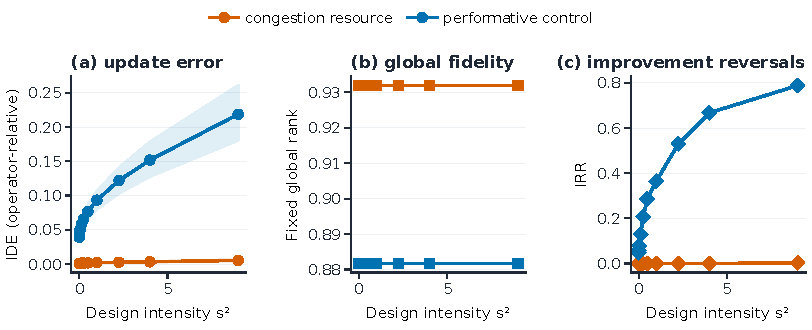
\includegraphics[width=\linewidth]{fig2_operator_shift.pdf}
  \caption{Operator shift exposes update-level failure. The horizontal axis
  is the design intensity $s^2$, not a measured $\chi^2$ divergence. Global
  Spearman rank is a fixed calibration reference.}
  \label{fig:operator-shift}
\end{figure}

Deployment response provides a distinct source of discrepancy. In the
strategic fixture, the strategic-minus-actor effect is
\StrategicEffect{} \StrategicEffectCI{}, with family-balanced strategic
reversal rate \StrategicReversalRate{}. A second Leduc confirmation cohort shows the
same mechanism along the response horizon: the proxy-positive reversal rate
rises from 2.5\% under one-step response to 51.7\% under eight-step adaptation
(Appendix~\ref{app:fidelity-response}). The appendix also compares
response-disabled proxy, actor, and strategic evaluations across opponents. Together,
these results identify two distinct sources of update-level failure: operator
shift can concentrate error on the transitions proposed by the improvement
process, while deployment response can sharply alter the value and sign of a
candidate after deployment.

\subsection{Decision Relevance and High-Fidelity Resolvability}
\label{sec:exp-decision}

Proposition~\ref{prop:decision-preservation} shows that update error changes a
replacement decision only when it is large relative to the candidate margin.
For each held-out root, we compare the deployment winner with its competitors
using a winner-relative correction-to-margin ratio; values above one indicate
disjoint proxy and deployment optimal sets, with one as the tie boundary.
Appendix~\ref{app:pivot-ext} gives the exact definition.

Across \RevisionDecisionRoots{} held-out roots, proxy and deployment optimal sets
are disjoint in \RevisionDecisionFlips{} cases. Figure~\ref{fig:decision-relevance}
shows that disagreement alone does not determine validation value: what matters
is whether the fidelity error is large enough to threaten the replacement
decision and whether available HF evidence can resolve the resulting margin.
At the primary long budget, the PIVOT query set intersects the ex-post
decision-critical pair in \RevisionCriticalQueryRate{}
\RevisionCriticalQueryRateCI{} of roots, while the mean model-assumed queried
observation standard deviation (SD) is \RevisionCriticalNoiseMargin{} \RevisionCriticalNoiseMarginCI{}
times the proxy top-2 margin. This regularized-model diagnostic does not
estimate HF observation noise directly; targeting alone need not resolve ordering.

\begin{figure}[!t]
  \centering
  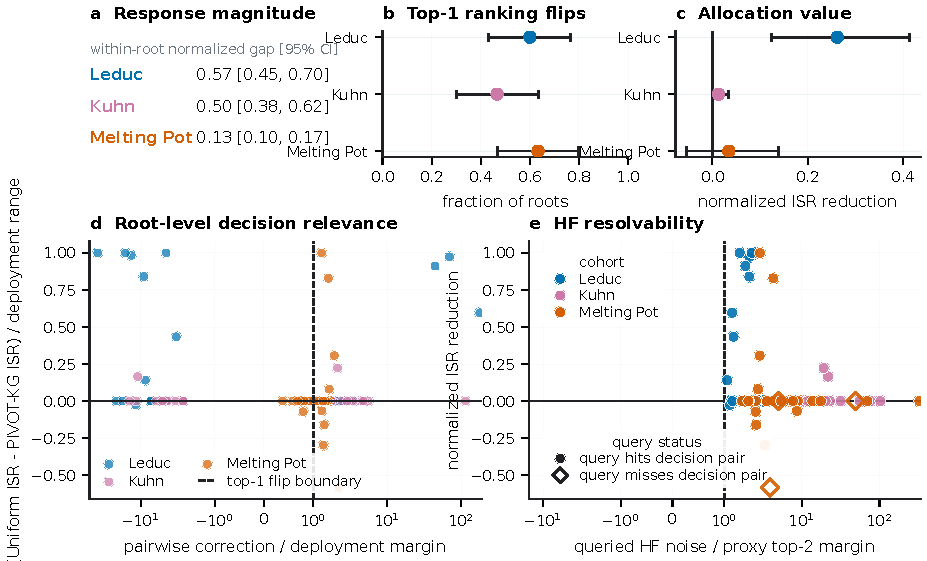
\includegraphics[width=\linewidth]{fig1_decision_relevance.pdf}
  \caption{Decision relevance and HF resolvability. (a) Disjoint optimal sets.
  (b) Winner-relative correction-to-margin ratio versus
  normalized ISR reduction. (c) Model-assumed observation SD relative to the
  proxy top-2 margin versus normalized ISR reduction; filled markers hit the ex-post
  decision-critical pair.}
  \label{fig:decision-relevance}
\end{figure}

The held-out analysis isolates the mechanism behind useful validation:
fidelity error must threaten the replacement decision, and the available HF
evidence must be informative enough to resolve that uncertainty.

\subsection{PIVOT-KG under Limited High-Fidelity Budgets}
\label{sec:exp-pivot}

Table~\ref{tab:latest-main} reports the primary held-out fixed-budget comparison.
PIVOT-KG substantially lowers ISR in Leduc, the contrast is small in Kuhn, and
the primary Melting Pot comparison is unresolved. This heterogeneity is
consistent with the preceding mechanism analysis: deployment response alone
does not determine the value of targeted validation. Secondary Melting Pot
conditions are reported in Appendix~\ref{app:pivot-ext}.
For these cohorts, PIVOT-KG and Uniform share the calibrated posterior,
observation-update rule, and final selection rule, differing only in query
allocation; related component diagnostics are reported in
Appendix~\ref{app:pivot-ext}.

\begin{table}[!ht]
  \centering
  \scriptsize
  \caption{Primary held-out fixed-budget comparisons (30 paired roots per row).
  Positive Uniform $-$ PIVOT means lower ISR for PIVOT-KG; brackets give 95\%
  root-bootstrap CIs.}
  \label{tab:latest-main}
  \begin{tabular}{@{}p{0.28\linewidth}rrrrp{0.15\linewidth}l@{}}
\toprule
World / condition & $n$ & Uniform ISR & PIVOT-KG ISR & Gain & 95\% CI & Interpretation \\
\midrule
Leduc, long / 2 queries (primary) & 30 & 0.046 & 0.009 & 0.036 & [0.014, 0.064] & positive \\
Kuhn, long / 2 queries (primary) & 30 & 0.058 & 0.056 & 0.002 & [0.000, 0.006] & near-null \\
Melting Pot, long / 2 queries (primary) & 30 & 1.742 & 0.836 & 0.906 & [-0.784, 3.401] & unresolved \\
Melting Pot, long / 1 query (secondary) & 30 & 1.742 & 1.859 & 3.423 & [0.390, 6.944] & positive \\
Melting Pot, short / 5 queries (sec.) & 30 & 1.035 & 1.610 & -0.575 & [-1.042, -0.180] & negative \\
\bottomrule
\end{tabular}

\end{table}

We also retain controlled batch-selector diagnostics, distinct from
Algorithm~\ref{alg:pivot-kg}. Their pooled candidate-only cumulative improvement-selection regret (CISR) contrast for Proxy-Only minus PIVOT-batch under the legacy forced-replacement setting is \ClosedLoopEffect{} \ClosedLoopEffectCI{}
over \ClosedLoopRounds{} rounds; Figure~\ref{fig:efficiency} compares the
single-decision batch selectors at matched query counts. A second Leduc
confirmation cohort yields a prespecified PIVOT-KG versus expected-Uniform
selected-gain contrast of +0.02989 using a repeated-query, sample-size variant.
Its component comparisons, the legacy closed-loop target, stopping behavior,
and numerical diagnostics are specified in Appendix~\ref{app:pivot-ext}.

\begin{figure}[!t]
  \centering
  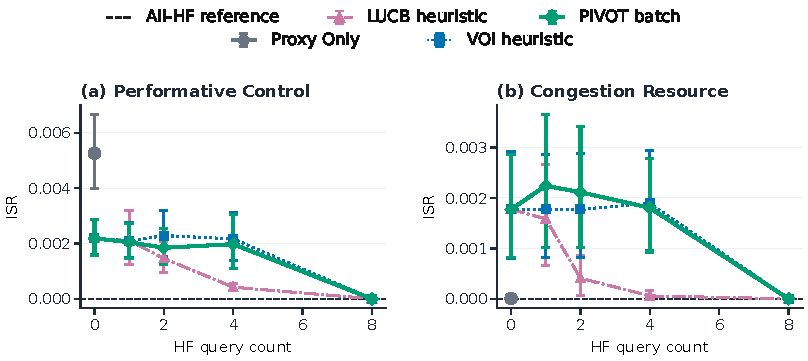
\includegraphics[width=\linewidth]{fig4_evidence_efficiency.pdf}
  \caption{Legacy batch-selector diagnostics at matched HF query counts in
  (a) Performative Control and (b) Congestion Resource. Lower single-decision
  ISR is better; the all-HF reference uses only fully queried rows.
  Intervals bootstrap seeds.}
  \label{fig:efficiency}
\end{figure}

Together, these results support the central prediction of our analysis:
decision-aware validation is most useful when the remaining uncertainty is
both consequential for the replacement decision and resolvable by the
available HF evidence.

\subsection{Reactive Driving Stress Test}
\label{sec:exp-highway}

We evaluate PIVOT-KG through saved-truth replay and fresh reactive-driving
simulator runs. The HighwayEnv saved-truth replay uses eight
scheduled candidates formed by crossing four non-idle actions with early and
late half-horizon windows, fits the correction model on 40 calibration roots,
and evaluates 120 disjoint test roots. At the primary budget $B=4$, PIVOT-KG
reduces ISR relative to the exact Uniform validation rule by
\HighwayRedesignBudgetFourContrast{} \HighwayRedesignBudgetFourCI{}.
The Uniform rule averages exactly over all feasible queried subsets. Queries
in this offline replay use saved deployment values and simulated observations;
they do not invoke new actor rollouts.

The HighwayEnv result shows the same decision-aware validation principle in
a reactive driving candidate-allocation problem. Two fresh HighwayEnv
simulator cohorts provide targeted-baseline context at $B=4$:
\begin{center}
\scriptsize
\setlength{\tabcolsep}{3pt}
\begin{tabular}{@{}p{2.0in}cc@{}}
\toprule
Cohort & IVR $-$ PIVOT-KG & Top-Proxy $-$ PIVOT-KG \\
\midrule
Fresh simulator (development; frozen calibration) & $-0.0030\ [-0.0073,0.0008]$ & $0.0135\ [0.0024,0.0307]$ \\
Independent calibration/test cohort & $0.0016\ [-0.0042,0.0071]$ & $-0.0001\ [-0.0050,0.0045]$ \\
\bottomrule
\end{tabular}
\end{center}
Positive values favor PIVOT-KG. IVR is inconclusive in both cohorts, and
Top-Proxy is positive in the first but null in the independent cohort; these
are single-decision simulator results. The secondary $B=2$ redesign result
and the earlier MetaDrive~\citep{li2022metadrive} stress test are reported in
Appendix~\ref{app:physical-stress}.

\paragraph{Exploratory MetaDrive PGMA boundary.}
In a 24-root development cohort, PIVOT-KG and IVR selected identical actions
(KG minus IVR $=0.000$), while all three KG--Top-Proxy disagreements favored
Top-Proxy (KG minus Top-Proxy $=-8.396448$); the calibration benefit
(Calibrated-No-HF minus Proxy-Only $=+26.8376$) reflects the calibrated prior,
not KG allocation. We retain this scripted-IDM, matched-start/common-seed
result as an exploratory boundary analysis, not confirmatory evidence of KG
superiority; full diagnostics are in Appendix~\ref{app:physical-stress}.

\subsection{Controlled Multi-round Replacement Loop}
\label{sec:controlled-multiround}

We also evaluated PIVOT-KG-Loop-v3c, a controlled five-round extension in
synthetic PerformativeWorld with a fixed proposer, four candidates, two paired
HF queries per round, and 120 fresh roots per response regime. This protocol
was selected after exploratory v1--v4a variants, and its six-test Holm
correction covers only the prespecified v3c contrasts. The paired results
favor PIVOT-KG-Loop-v3c in this controlled extension, not in submitted static
Algorithm~\ref{alg:pivot-kg} or general self-improvement; the Appendix reports
the means, intervals, and calibration/test-shift diagnostics
(Appendix~\ref{app:pivot-ext}).


\FloatBarrier
\section{Conclusion}

Improvement Fidelity is our core contribution: an operator-relative target for
whether a proposed update remains beneficial after deployment response. Our
analysis shows that global policy accuracy alone cannot ensure this; operator
shift and candidate margins determine whether fidelity errors change a
replacement decision. PIVOT is the paired validation framework, and PIVOT-KG
applies established KG to allocate HF evidence by replacement regret. Results
support conditional value in controlled, multi-agent, and driving studies;
fresh HighwayEnv simulator cohorts show no significant advantage over IVR.

Evidence depends on a calibrated correction prior and informative HF queries;
reported intervals condition on fitted calibration data. The response models
and virtual driving studies do not span deployment dynamics. The five-round
v3c result is a controlled post-search extension with calibration/test shift,
not confirmation of static Algorithm 1 or general self-improvement. Future
work should study cross-round calibration and intervention-based HF evaluation.
We make no claim of universal KG superiority, equilibrium convergence, or
physical-driving performance.

\label{sec:conclusion-end}


\subsection*{AI use statement}
The authors developed the problem formulation, theoretical contributions, and
initial experiments. During the review response, generative AI tools assisted
with experiment implementation and audit code, research analysis, and language
polishing. Generative AI tools also assisted with review-stage experimental
design and protocol refinement. The authors independently reviewed the
protocols and results,
verified the reported evidence, and take full responsibility for the research
and final manuscript.

\subsection*{Ethics statement}
This study uses controlled virtual environments and publicly available
benchmark environments and data. It involves no human subjects, personal data,
live trading, or real-world autonomous-system deployment. The experiments are
conducted entirely in simulation and do not directly affect users or physical
systems.

\subsection*{Reproducibility statement}
The accompanying supplementary material includes an anonymized code archive,
cohort-specific configurations, figure provenance, and reproduction
instructions for the reported results, distinguishing legacy batch diagnostics
from the held-out and driving implementations.
The anonymized code and reproducibility materials are also available at
\url{https://anonymous.4open.science/r/pivot-anonymous-review-2E67/}.

\label{refs:start}
\bibliographystyle{iclr2027_conference}
\bibliography{references}

\clearpage
\appendix
\label{app:artifact}

\section{Response Mechanism Analyses}
\label{app:fidelity-response}

The operator contrast pools Performative Control, Congestion Resource, and
frozen Multi-Agent Particle Environment 2 (MPE2)~\citep{lowe2017maddpg}
with weights $0.4/0.4/0.2$; Figure~\ref{fig:operator-shift} shows the
first two. Its interval resamples 450 condition/seed cells sharing 30 seeds;
figure bands resample six condition means. Congestion strengths are duplicated;
global rank is a fixed zero-shift evolutionary-policy reference. These are
descriptive shift diagnostics, not measured $\chi^2$ divergence.
Figure~\ref{fig:layers}'s proxy disables response, unlike the fixed-incumbent-world
$\Delta_{\mathrm{direct}}$. Strategic reversal averages the three adaptive families.

\begin{figure}[!htbp]
  \centering
  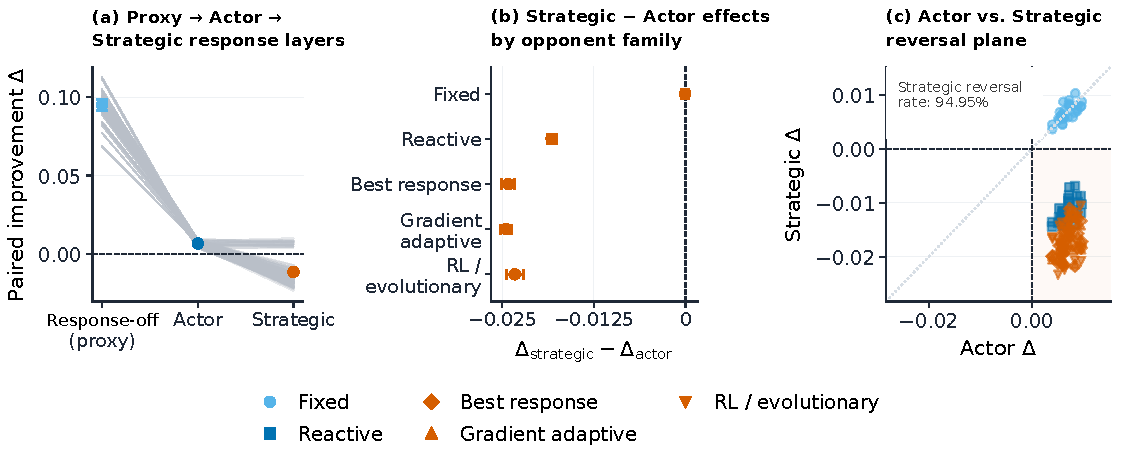
\includegraphics[width=\linewidth]{figA_response_footprint.pdf}
  \caption{Response mechanisms. (a) Response-disabled proxy, actor, and
  strategic evaluations. (b) Strategic-minus-actor effects by opponent family. (c) Actor
  versus strategic improvement. Intervals use 30 matched seeds.}
  \label{fig:layers}
\end{figure}

A separate Leduc confirmation cohort tests the same mechanism along the
response horizon. Among proxy-positive candidates, the mean root-level
improvement-reversal rate rises from 2.5\% under one-step response to 51.7\%
under eight-step adaptation (Figure~\ref{fig:leduc-response-horizon}). This
supports the main-text conclusion that deployment response can amplify
update-level failure rather than merely shift policy values uniformly.

\begin{figure}[!htbp]
  \centering
  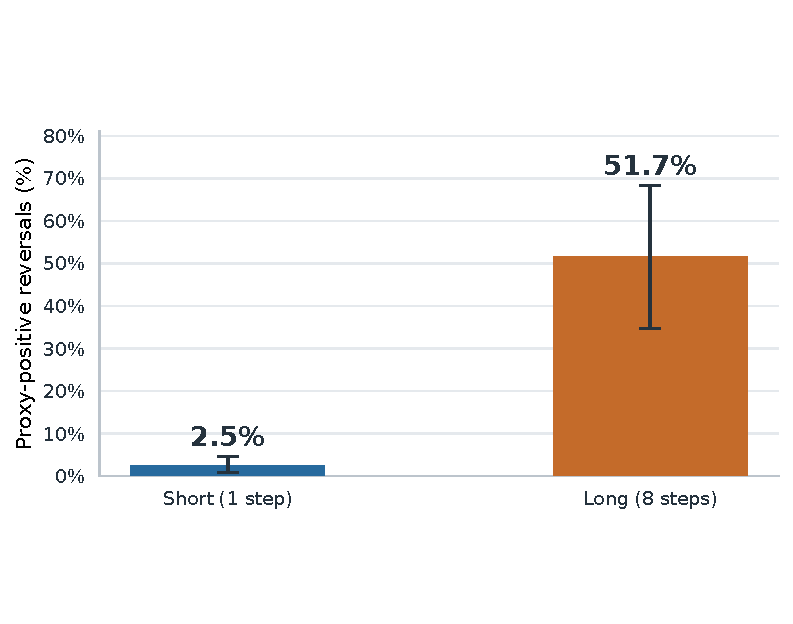
\includegraphics[width=0.70\linewidth]{figures/additional_leduc/01_proxy_deployment_reversal.pdf}
  \caption{Leduc response-horizon confirmation. Reversal rates are computed
  among proxy-positive updates within each root, where a reversal means
  negative deployment gain. Bars show means across 30 roots under one-step
  and eight-step adaptation, with 95\% root-bootstrap CIs.}
  \label{fig:leduc-response-horizon}
\end{figure}

\FloatBarrier
\section{Extended PIVOT-KG Evaluation}
\label{app:pivot-ext}

In the calibrated poker, Melting Pot, and driving evaluations, candidate
coordinates follow the same fixed update slots across calibration and test roots.

\paragraph{Decision diagnostics.}
Let $T=\arg\max_{C^+}\Delta_*$ and $b\in\arg\max_{j\in T}\Delta_{V,j}$.
The ratio is $\max_{k\notin T}(G_b-G_k)/(\Delta_{*,b}-\Delta_{*,k})$,
with $G=\Delta_*-\Delta_V$ and tie tolerance $10^{-12}$.
The 51 disagreements are disjoint optimal sets; 28 roots have tied optima.
Above one indicates disjoint optimal sets; one is the tie boundary.
The query-hit pair uses proxy/deployment top candidates within $C$ (stable index ties);
top-2 margins exclude no-update. Normalization divides Uniform minus PIVOT ISR
by the deployment range over $C^+$. The noise ratio uses mean queried $\sqrt{R_j}$,
a margin floor of $10^{-12}$, and poker's model-variance floor $0.25$;
it is model-assumed, not directly measured observation noise.

At the primary long budget, the decision-critical query-hit rates are
\RevisionLeducCriticalQueryRate{} in Leduc,
\RevisionKuhnCriticalQueryRate{} in Kuhn, and
\RevisionMeltingCriticalQueryRate{} in Melting Pot. The descriptive normalized
gain is \RevisionCriticalQueryHitGain{} \RevisionCriticalQueryHitGainCI{}
among the 87 hit roots and
\RevisionCriticalQueryMissGain{} \RevisionCriticalQueryMissGainCI{} among the
three misses. These diagnostics separate successful targeting from successful
resolution.

\paragraph{Secondary and confirmation analyses.}
The first cohorts use 12 calibration/30 test roots and one frozen Uniform
draw. Poker has nine alpha-mixture candidate slots, including an alpha=0
incumbent copy, plus a separate no-update action; Melting Pot
uses eight specialist mixtures on one repeated stag-hunt substrate. Full
candidate/cost protocols accompany the supplement. The designated allocation
interaction is the paired long-minus-short contrast
$(\mathrm{ISR}_{U}-\mathrm{ISR}_{P})_{\rm long}-(\mathrm{ISR}_{U}-\mathrm{ISR}_{P})_{\rm short}$:
$0.0365\,[0.0145,0.0637]$ (Leduc), $0.0020\,[0,0.0058]$ (Kuhn), and
$1.4815\,[-0.3930,4.0956]$ (Melting Pot); only Leduc meets the joint
primary/interaction criterion.

Table~\ref{tab:secondary-sealed} retains the secondary comparisons. The second
Leduc cohort was designed after the first-cohort results, with fresh confirmation
roots. This cohort is a mechanism confirmation study rather than a direct replication of the fixed-budget benchmark. Its PIVOT-KG variant queries $(j,n)$ pairs with $n\in\{512,2048,4096\}$,
permits repeated candidates, and charges $2n$ hands; it extends the once-per-candidate
Algorithm~\ref{alg:pivot-kg}. At 16,384 hands its prespecified contrast against
exact-subset expected Uniform is +0.02989 under long adaptation.
Figure~\ref{fig:leduc-components} retains the component comparisons; its final
row is $(\mathrm{PIVOT}-\mathrm{Uniform})_{\rm long}-(\mathrm{PIVOT}-\mathrm{Uniform})_{\rm short}$,
not a direct long-minus-short policy-gain contrast.

\begin{table}[!htbp]
  \centering
  \footnotesize
  \caption{Secondary held-out comparisons. Positive Uniform $-$ PIVOT means
  lower ISR for PIVOT-KG; brackets give 95\% root-bootstrap CIs.}
  \label{tab:secondary-sealed}
  \begin{tabular*}{\linewidth}{@{\extracolsep{\fill}}lcrrl@{}}
\toprule
World / response & HF queries & Uniform ISR & PIVOT-KG ISR & \shortstack[l]{Uniform $-$ PIVOT\\{[95\% CI]}} \\
\midrule
Melting Pot, long & 1 & 5.283 & 1.859 & 3.423 [0.390, 6.944] \\
Melting Pot, short & 5 & 1.035 & 1.610 & -0.575 [-1.042, -0.180] \\
\bottomrule
\end{tabular*}

\end{table}

\begin{figure}[!htbp]
  \centering
  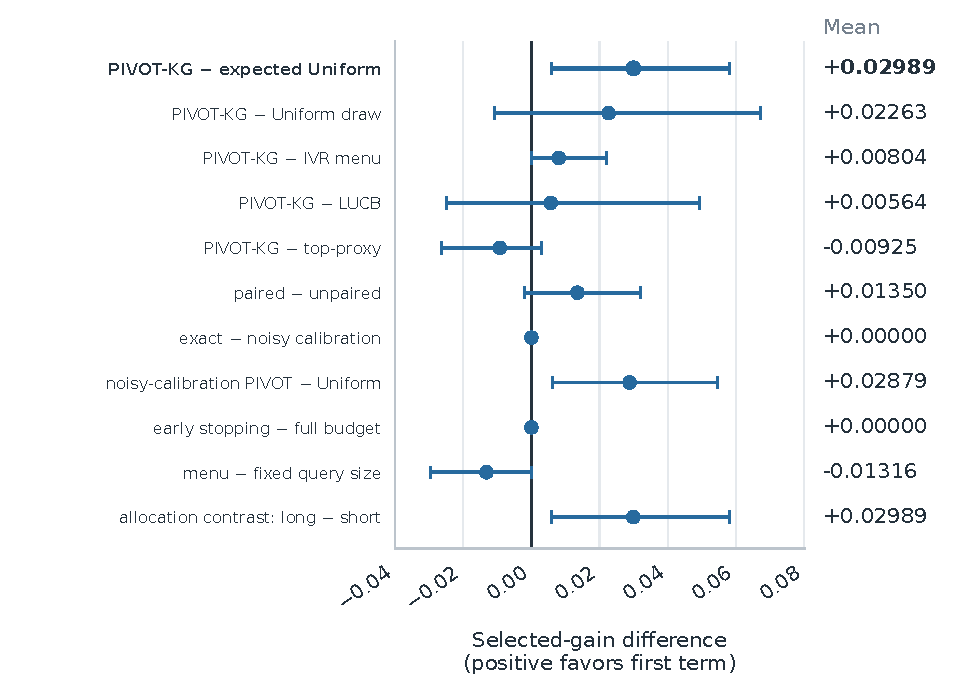
\includegraphics[width=\linewidth]{figures/additional_leduc/05_v4_component_contrasts.pdf}
  \caption{Leduc confirmation-cohort component contrasts under long response
  (30 roots; primary budget 16,384 HF hands). Positive values favor the first
  term. The expected-Uniform comparison is prespecified primary; all others
  are secondary with unadjusted 95\% CIs.}
  \label{fig:leduc-components}
\end{figure}

The secondary stopping rule reduces mean HF use from 16,384 to 12,083.2 hands,
a 26.25\% reduction, while producing the same selected gain as the full-budget
rule on all 30 observed roots. The paired difference in HF use is $-4300.8$
$[-6007.5,-2662.4]$ hands. Thus the stopping variant can save validation
queries in this cohort without changing the observed replacement decision.

\paragraph{Post-review Poker calibration resampling.}
We refit the default correction prior in 500 bootstrap resamples of the
existing 12-root Leduc calibration cohort and replayed the selectors on the
same 30 held-out roots. Uniform-minus-PIVOT ISR remained positive in all fits
(median $0.0365$; 2.5th--97.5th calibration-refit percentiles
$[0.0228,0.1127]$), while the IVR-minus-PIVOT ISR contrast was zero in every
fit. This resampling range is conditional on the fixed test cohort; it is not
an independent calibration cohort or a new rollout.

\paragraph{Earlier loop variants.}
The initial 30-root v1 loop gave cumulative ISR 2.602 for PIVOT-KG versus
1.986 for IVR and 1.999 for Top-Proxy; paired 95\% intervals crossed zero.
The v2 confirmation (120 roots per response regime) gave PIVOT/IVR/Top-Proxy
cumulative ISR of 0.0296/0.0669/0.1331 (low), 0.3497/0.5770/0.1600
(medium), and 0.2763/0.3548/0.3048 (high): PIVOT beat both at low, beat IVR
but lost to Top-Proxy at medium, and had inconclusive ISR contrasts and lower
deployment utility than both baselines at high.
The initial v3 run is excluded because its implementation treated noisy HF
observations as exact. Corrected v3b retained a common sentinel and online
coefficient updates and was mixed against Top-Proxy. The v4a development run
lost to Top-Proxy in all three response regimes and was not promoted. These
variants and their ledgers remain in the audit archive and are not pooled with
the v3c result.

\paragraph{PIVOT-KG-Loop-v3c confirmation.}
The amended PerformativeWorld study uses five rounds, four candidates, two
sequential paired HF queries per round, and 120 fresh roots in each low,
medium, and high response regime. The three methods share the calibration data,
proposer function and random-seed schedule, contextual linear correction model,
response operator, terminal posterior-mean selector, and total query budget.
Their first-round panels match; later panels are generated relative to each
method's own incumbent and may diverge. The amended protocol removes the
sentinel: both queries are allocated by each method's own acquisition rule.
Relative to v3b, v3c changes both the sentinel-query allocation and the
cross-round correction-model update policy; it is therefore a protocol-level
extension, not an isolated sentinel ablation. The correction model is reset
each round; previous-round HF observations do not update its regression. Thus
the IVR and Top-Proxy \texttt{Online} labels mean
within-round sequential posterior conditioning, not persistent online
calibration. The extension is not the submitted static
Algorithm~\ref{alg:pivot-kg}.

Fresh confirmation roots are conditional on the protocol selected after
exploratory variants; Holm correction covers the six prespecified within-v3c
contrasts, not the preceding v1--v4a search. The confirmation means and paired
intervals are reported in Table~\ref{tab:multiround-confirmation}. The six paired baseline-minus-PIVOT intervals exclude zero. No
sampled sign flip was as extreme as the observed contrast in 100,000 draws;
the plus-one estimate is approximately $10^{-5}$ per test and the six-test
Holm-adjusted value is approximately $6\times10^{-5}$. PIVOT-minus-IVR
cumulative deployment-return differences are
$0.0757\,[0.0647,0.0878]$, $0.4530\,[0.3666,0.5606]$, and
$1.3656\,[0.9790,1.8314]$ in low/medium/high response. The corresponding
PIVOT-minus-Top-Proxy intervals are
$0.0643\,[0.0489,0.0798]$, $0.1830\,[0.1429,0.2236]$, and
$0.1863\,[0.1457,0.2304]$. Thus the deployment-return criterion is also
positive in all six comparisons.

The correction model's calibration pressure support is $[0.054,0.696]$.
Outside-support test states occur in 0/1800, 148/1800 (8.2\%), and 423/1800
(23.5\%) ledger rows under low/medium/high response. At medium response,
PIVOT-KG-Loop-v3c has 0/600 such states, compared with 76/600 for IVR and 72/600 for
Top-Proxy; at high response the counts are 83/600, 163/600, and 177/600.
These distributions arise on method-induced trajectories. The counts describe
extrapolation on some paths, but do not identify its causal effect on ISR.
Across test candidate vectors, 80.3\% and 80.0\% exceed the calibration-set
Mahalanobis distance thresholds at P95 and P99, respectively. The calibration
feature \texttt{round\_fraction} is fixed at zero while tests span $[0,1]$.
The calibration feature for round fraction is constant in calibration
(round zero), so its later-round effect is not identified by training data.
Five-fold root-held-out calibration gives 93.0\% working 95\% interval
coverage; this does not establish coverage for OOD deployment states. We report
these limits with the positive result. The independent replay
recomputed all 5,400 round records, 10,800 HF observations, 5,400 independent
evaluation panels, and 5,400 deployment returns; all protocol checks passed.
The complete source hashes, pressure-support audit, and ledgers are included
in the supplementary audit record. This result is conditional on the declared
controlled world, candidate proposer, calibration cohort, and five-round
horizon; it does not establish physical-driving or universal superiority.

\begin{table}[!htbp]
  \centering
  \scriptsize
  \setlength{\tabcolsep}{4pt}
  \caption{PIVOT-KG-Loop-v3c five-round confirmation (120 paired roots per
  response regime). ISR is cumulative improvement-selection regret; lower is
  better. Contrasts are baseline minus PIVOT-KG-Loop-v3c with paired 95\%
  root-bootstrap confidence intervals. Holm correction covers the six
  prespecified contrasts shown here only.}
  \label{tab:multiround-confirmation}
  \begin{tabular}{lrrrrr}
    \toprule
    Response & PIVOT ISR & IVR ISR & IVR $-$ PIVOT [95\% CI] & Top-Proxy ISR & Top-Proxy $-$ PIVOT [95\% CI] \\
    \midrule
    Low    & 0.00888 & 0.05574 & 0.0469 [0.0385, 0.0565] & 0.07095 & 0.0621 [0.0491, 0.0755] \\
    Medium & 0.00141 & 0.44046 & 0.4391 [0.3706, 0.5168] & 0.23241 & 0.2310 [0.1805, 0.2823] \\
    High   & 0.08886 & 0.98532 & 0.8965 [0.6449, 1.1897] & 0.33346 & 0.2446 [0.2019, 0.2917] \\
    \bottomrule
  \end{tabular}
\end{table}

\paragraph{Frozen-state matched diagnostic.}
To isolate query allocation from path divergence, a separate auxiliary study
held the initial state, incumbent, candidate panel, proxy values, calibration,
budget, evaluation seeds, and terminal rule fixed across selectors (120 roots
per response regime). At low response, all methods had zero mean ISR. At
medium response, mean ISR was 0.00054 for the v3c KG selector, 0.19957 for IVR, and
0.06443 for Top-Proxy; baseline-minus-PIVOT paired 95\% intervals were
$[0.1763,0.2214]$ and $[0.0496,0.0788]$. At high response, the KG selector had ISR
0.03297 versus 0.03051 for IVR (difference $-0.00246$,
$[-0.0152,0.0105]$, inconclusive) and 0.09510 for Top-Proxy (difference
$0.06213$, $[0.0497,0.0751]$). Holm-adjusted tests cover these six auxiliary
contrasts only. This post-review diagnostic is not pooled with v3c and does
not correct for the preceding variant search; it supports selector benefits
under some fixed states, not a universal KG advantage. Its preregistration,
ledger, and independent replay are included in the supplement.

\paragraph{Closed-loop and numerical diagnostics.}
Figures~\ref{fig:efficiency}, \ref{fig:closed-loop}, and~\ref{fig:robustness}
use legacy batch selection, not Algorithm~\ref{alg:pivot-kg}: no within-batch
reacquisition; observed values replace queried estimates; unqueried estimates
can omit later observations. The closed loop forces replacement and reports
$\mathrm{CISR}_C=\sum_t[\max_{j\in C_t}\Delta_{*,j}-\Delta_{*,\hat j_t}]$
without no-update; negative improvement with zero regret is then possible.
Figure~\ref{fig:efficiency} counts queries and uses VOI/LUCB heuristics.
Figure~\ref{fig:robustness} compares Monte Carlo draws on 24 Congestion test
groups ($K=4$): all costs scale equally, query count stays two, and seeds vary.
With common draws the ranking is invariant, so this does not identify cost misspecification.

\begin{figure}[!htbp]
  \centering
  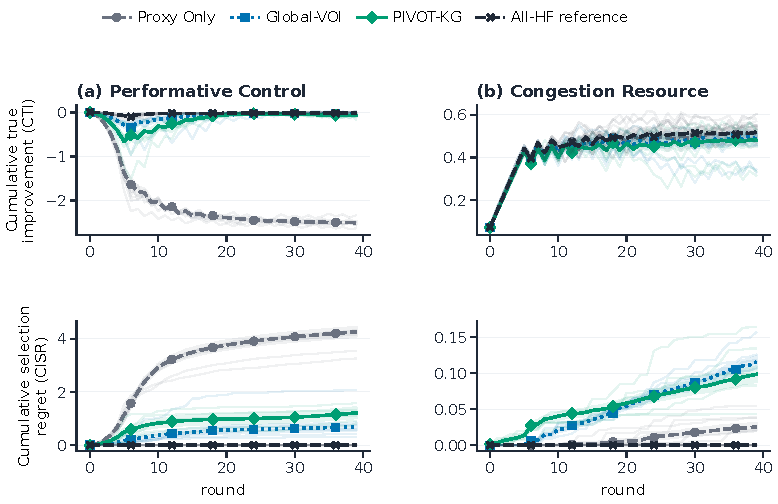
\includegraphics[width=\linewidth]{fig5_closed_loop.pdf}
  \caption{Legacy forced-replacement trajectories. Top: cumulative true
  improvement; bottom: candidate-only $\mathrm{CISR}_C$, excluding no-update.
  Thin curves are seeds; markers summarize batch decision rules.}
  \label{fig:closed-loop}
\end{figure}

\begin{figure}[!htbp]
  \centering
  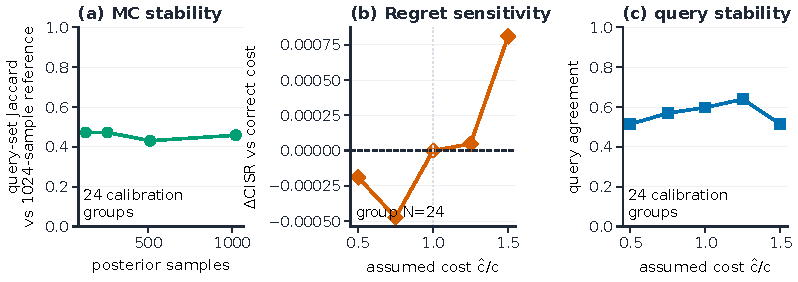
\includegraphics[width=\linewidth]{figC_posterior_robustness.pdf}
  \caption{Legacy batch-selector Monte Carlo diagnostics on 24 test groups.
  Panels show query agreement across sample counts and regret/query variation
  under common cost scaling with different random draws; this is not an
  identified cost-misspecification effect.}
  \label{fig:robustness}
\end{figure}

Additional response-mixture settings yield positive, null, and negative
allocation effects, consistent with the main-text conclusion that deployment
response alone does not determine validation value. Full method-by-method and
response-mixture diagnostics are provided in the supplement.

\FloatBarrier
\section{Reactive Driving Stress Tests}
\label{app:physical-stress}
\label{app:highway-replication}

\paragraph{HighwayEnv.}
The original and fresh-seed five-action cohorts, together with their paired
root-bootstrap intervals, are retained in the supplementary audit. The
eight-candidate redesign uses 40 calibration roots, 120 disjoint test roots,
exact-subset Uniform, and saved-truth offline replay; all smoke-exposed roots
remain included without retuning. This is the source of the 0.0435 to 0.0055
ISR comparison; it is distinct from the new simulator runs below.

The fresh simulator development cohort reuses the frozen calibration model
and gives IVR-Trace, Top-Proxy, and sampled-Uniform
baseline-minus-PIVOT ISR contrasts of $-0.0030$, $0.0135$, and $0.0295$;
the independent calibration/test cohort gives $0.0016$, $-0.0001$, and $0.0167$.
Their paired intervals and simulator-call accounting are in the supplement.
Both are single-decision evidence within the same HighwayEnv task, not evidence
of universal KG superiority or multi-round co-adaptation.

\paragraph{Earlier MetaDrive stress cohort.}
We additionally evaluate an earlier MetaDrive~\citep{li2022metadrive} cohort under
a long-response condition with 12 profiles and 30 held-out roots. Its
prespecified $B=2$ PIVOT-KG--Uniform contrast is
$+1.89\,[-1.29,5.49]$, unresolved; $B=1,4$ are secondary. We retain this
boundary result and its full cost breakdown in the supplement.

\paragraph{Exploratory MetaDrive PGMA allocation-development boundary.}
The later PGMA allocation-development study retains all 24 declared roots with
$K=4$ and $B=2$, shared panel/prior/observation model/terminal rule, and an
independent truth bank. KG and IVR select the same action on every root (KG
minus IVR $=0.000$). KG and Top-Proxy disagree on three roots, all favoring
Top-Proxy, giving KG minus Top-Proxy $=-8.396448$. Calibrated-No-HF minus
Proxy-Only is $+26.8376$; this is calibration value, not KG allocation value.
The opponents are scripted IDM policies, and pairing is matched-start/
common-seed rather than strict CRN. This is descriptive development evidence,
not a confirmatory superiority result; the complete decision and truth ledgers
are included in the external audit archive.

\paragraph{Evaluator boundary.}
Improvement Fidelity defines an evaluation target, not a preferred learner
architecture. In an out-of-distribution comparison, a transition-specific
learner does not outperform the global learner: the transition-minus-global
ISC contrast is \OODGain{} \OODGainCI{}. Full ISC and IDE comparisons are
reported in the supplement.


\begin{figure}[!htbp]
  \centering
  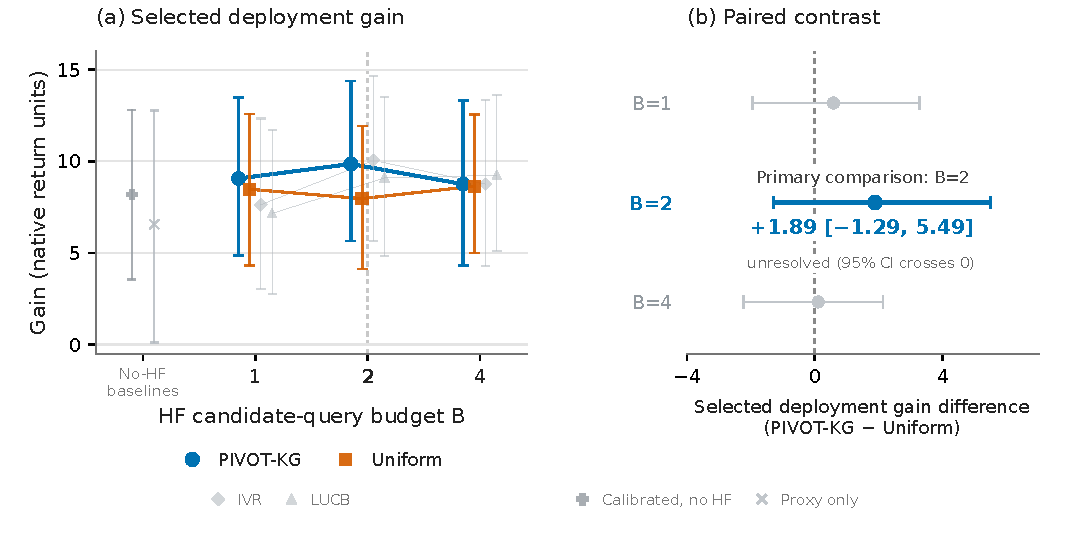
\includegraphics[width=\linewidth]{figures/additional_metadrive/matched_posterior_selected_audit_gain.pdf}
  \caption{Earlier MetaDrive stress test as a boundary case. The prespecified $B=2$
  comparison remains unresolved: $+1.89\,[-1.29,5.49]$, with the 95\%
  root-bootstrap CI crossing zero. (a) Selected deployment gain (12 profiles,
  30 held-out roots; marginal 95\% root-bootstrap intervals).
  (b) Paired PIVOT-KG--Uniform selected deployment gain contrasts;
  $B=1,4$ are secondary.}
  \label{fig:metadrive-stress}
\end{figure}
\end{document}
